% Build from docs/manual with pdflatex qstab_manual.tex (twice).
% guide_ranges.tex is generated from the checked-in example markers.
\documentclass[11pt,a4paper]{article}
\usepackage[T1]{fontenc}\usepackage{textcomp,upquote}\usepackage{lmodern,microtype,amsmath,amssymb}
\usepackage[margin=22mm,top=23mm,bottom=21mm]{geometry}
\usepackage{xcolor,booktabs,tabularx,array,listings,tikz,fancyhdr,hyperref}
\definecolor{ink}{HTML}{143344}\definecolor{teal}{HTML}{006D75}\definecolor{soft}{HTML}{EFF5F4}
\definecolor{warm}{HTML}{A24D1C}\definecolor{muted}{HTML}{465E69}
\hypersetup{colorlinks=true,linkcolor=teal,urlcolor=teal,pdftitle={qstab: A public guide to quaternionic stability},pdfauthor={qstab project}}
\pagestyle{fancy}\fancyhf{}\fancyhead[L]{\sffamily\small\color{muted}qstab\enspace |\enspace Public guide}\fancyhead[R]{\sffamily\small\color{muted}Scalar polynomials and right spectra}\fancyfoot[R]{\sffamily\small\thepage}
\setlength{\headheight}{14pt}\setlength{\parindent}{0pt}\setlength{\parskip}{4pt plus 1pt}\renewcommand{\arraystretch}{1.18}
\newcolumntype{Y}{>{\raggedright\arraybackslash}X}
\lstset{upquote=true,language=Matlab,basicstyle=\ttfamily\small,keywordstyle=\color{teal}\bfseries,commentstyle=\color{muted},backgroundcolor=\color{soft},frame=single,rulecolor=\color{soft},columns=fullflexible,keepspaces=true,breaklines=true,showstringspaces=false,xleftmargin=4pt,xrightmargin=4pt,aboveskip=7pt,belowskip=4pt}
\ExplSyntaxOn
\newcommand{\m}[1]{
  \group_begin:
  \tl_set:Nn \l_tmpa_tl {#1}
  \tl_replace_all:Nnn \l_tmpa_tl {'}{\textquotesingle{}}
  \texttt{\tl_use:N \l_tmpa_tl}
  \group_end:
}
\ExplSyntaxOff
\newcommand{\HH}{\mathbb H}\newcommand{\CC}{\mathbb C}\newcommand{\RR}{\mathbb R}
\newcommand{\lead}[1]{\par\smallskip\noindent{\sffamily\bfseries\color{teal}#1}\enspace}
\newcommand{\unit}{\mathrm{i}}\newcommand{\qj}{\mathrm{j}}\newcommand{\qk}{\mathrm{k}}\newcommand{\ii}{\iota}
\newcommand{\topic}[2]{\clearpage\section{#1}\label{#2}}
% Generated by build_ranges.py from examples/qstab_guide_example.m
\expandafter\def\csname LabG01\endcsname{\lstinputlisting[firstline=30,lastline=34]{../../examples/qstab_guide_example.m}}
\expandafter\def\csname LabG02\endcsname{\lstinputlisting[firstline=39,lastline=45]{../../examples/qstab_guide_example.m}}
\expandafter\def\csname LabG03\endcsname{\lstinputlisting[firstline=50,lastline=55]{../../examples/qstab_guide_example.m}}
\expandafter\def\csname LabG04\endcsname{\lstinputlisting[firstline=60,lastline=67]{../../examples/qstab_guide_example.m}}
\expandafter\def\csname LabG05\endcsname{\lstinputlisting[firstline=72,lastline=79]{../../examples/qstab_guide_example.m}}
\expandafter\def\csname LabG06\endcsname{\lstinputlisting[firstline=84,lastline=95]{../../examples/qstab_guide_example.m}}
\expandafter\def\csname LabG07\endcsname{\lstinputlisting[firstline=100,lastline=110]{../../examples/qstab_guide_example.m}}
\expandafter\def\csname LabG08\endcsname{\lstinputlisting[firstline=115,lastline=121]{../../examples/qstab_guide_example.m}}
\expandafter\def\csname LabG09\endcsname{\lstinputlisting[firstline=126,lastline=130]{../../examples/qstab_guide_example.m}}
\expandafter\def\csname LabG10\endcsname{\lstinputlisting[firstline=135,lastline=141]{../../examples/qstab_guide_example.m}}
\expandafter\def\csname LabG11\endcsname{\lstinputlisting[firstline=146,lastline=154]{../../examples/qstab_guide_example.m}}

\newcommand{\lab}[1]{\lead{Executable example #1}\m{qstab\_guide\_example('#1')}\par\csname Lab#1\endcsname}
\begin{document}
\thispagestyle{empty}
{\color{teal}\sffamily QUATERNIONIC SYSTEMS AND CONTROL}\par\vspace{17mm}
{\sffamily\bfseries\color{ink}\fontsize{48}{50}\selectfont qstab}\par\vspace{5mm}
{\sffamily\fontsize{25}{30}\selectfont A public guide to\\quaternionic stability}\par\vspace{9mm}
{\Large Scalar polynomial families, right matrix spectra,\\ and numerical evidence in MATLAB}\par\vspace{6mm}
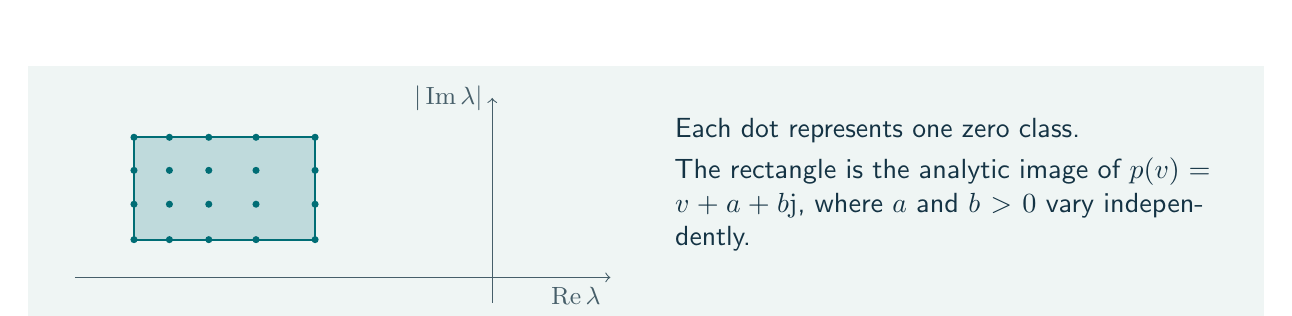
\begin{tikzpicture}[x=1cm,y=1cm]
\fill[soft] (0,0) rectangle (15.7,3.3);
\draw[muted,->] (0.6,0.62)--(7.4,0.62) node[below left]{\small $\operatorname{Re}\lambda$};
\draw[muted,->] (5.9,0.3)--(5.9,2.9) node[left]{\small $|\operatorname{Im}\lambda|$};
\fill[teal!25] (1.35,1.1) rectangle (3.65,2.4);\draw[teal,thick] (1.35,1.1) rectangle (3.65,2.4);
\foreach \x in {1.35,1.8,2.3,2.9,3.65}{\foreach \y in {1.1,1.55,1.98,2.4}{\fill[teal] (\x,\y) circle (.045);}}
\node[anchor=west,align=left,text width=6.9cm] at (8.1,1.8){\sffamily\color{ink}Each dot represents one zero class.\\[3pt]The rectangle is the analytic image of $p(v)=v+a+b\qj$, where $a$ and $b>0$ vary independently.};
\end{tikzpicture}
\vfill
\lead{Read with MATLAB open} All eleven numbered experiments have an executable key. They use real arrays or ordinary component structures and require no quaternion class. The same interfaces accept native MATLAB quaternion data.\par
\vspace{6mm}{\sffamily Public release 0.18.0 \enspace / \enspace 9 November 2026}\par
{\small\color{muted}MATLAB R2024b Update 2: all 693 checks passed on candidate 0.18.0-rc.1.
The numerical routines and examples are unchanged in this release.}\par
\clearpage
\tableofcontents
\bigskip
\lead{Example key} In the Command Window enter \m{qstab\_guide\_example('G04')}, replacing \m{G04} with the question you want to explore.
\par\smallskip\begin{tabularx}{\linewidth}{@{}lYlY@{}}\toprule
Key & Experiment & Key & Experiment\\\midrule
G01 & Algebraic zero vs. point value & G07 & Six-generator cubic from the paper\\
G02 & Delay reversal with grade & G08 & Certificate and witness\\
G03 & Matrix right eigenpairs & G09 & Ball vs. component box\\
G04 & First loss and later re-entry & G10 & Explore a random interval\\
G05 & Line vs. independent box & G11 & Physical window and global radius\\
G06 & Coarse and localized hulls &&\\\bottomrule
\end{tabularx}\par
\vfill\lead{Three routes} For a first run read Sections~\ref{sec:start}--\ref{sec:nominal}. For a polytopic study begin with Sections~\ref{sec:families}, \ref{sec:poly} and~\ref{sec:paper}. For existing project data use the function directory at the end, then consult the named MATLAB help entry for options.
\topic{Install, run and inspect}{sec:start}
Unpack the distribution into a writable folder. Open the directory containing \m{qstab\_setup.m}; it is the package root. In a normal public MATLAB session:
\begin{lstlisting}
qstab_setup('Examples',true);
qstab.about
catalogue = qstab_guide_example('list');
R = qstab_guide_example('G06');
R.ranges
\end{lstlisting}
The rows should be $[-3,5]$, $[1,5]$, $[1,5]$. This one call exercises an actual value-set calculation and two levels of enclosure. To run all eleven short examples without opening figures, use \m{A=qstab\_guide\_example('all');}. Results are returned in memory; \m{A\{6\}.ranges} retrieves the same rows. These examples write no files. Most pages reproduce the body of an experiment directly from its MATLAB source. To see the whole file, use \m{type qstab\_guide\_example}. Section~\ref{sec:paper} includes its own generator construction in that source.
\lead{Which software is needed?} Base MATLAB is sufficient for numeric arrays and ordinary component structures in these examples. The optional native input form uses the MathWorks \href{https://www.mathworks.com/help/fusion/ref/quaternion.html}{quaternion class}: use \m{which quaternion -all} to confirm which implementation your MATLAB finds. For example, Sensor Fusion and Tracking Toolbox provides this class; install a supported licensed product using MATLAB's Add-On Explorer. The active class should resolve under \m{matlabroot}. For large matrix Lyapunov solves the relevant Control System Toolbox functions may be useful. See \m{docs/installation.md} for product links and the optional external eigenvalue comparison. No external quaternion package, compiler, or download is needed for the guide. Avoid putting unrelated toolboxes on the search path to make these examples work.
\lead{Check the installation} The package has a separate, fuller acceptance test. Run it in a fresh MATLAB session from the package root:
\begin{lstlisting}
report = run_qstab_public;
report.archiveFile
assert(report.ok,'See the saved report: %s',report.archiveFile)
\end{lstlisting}
Unlike the examples, this command writes results: the named ZIP contains \m{report.txt} and \m{report.mat}. Copy an old report first if you want to retain it. The launcher temporarily restricts the search path and restores the caller's path and current directory. It does not edit the startup file. Native quaternion and graphics coverage require the corresponding MATLAB facilities. If a reader only wants the portable examples, \m{qstab\_guide\_example('all')} is the shorter entry point.
\lead{Optional external comparison} For an independently installed right eigensolver, add only its entry directory to the session path, inspect \m{which qeig -all}, then pass its handle explicitly to \m{run\_qstab\_eigen\_comparison} as \m{'LegacyFunction',@qeig}. This is separate from public acceptance. The author's \href{https://github.com/michaelsebek/qpe-public}{qpe-public} deals with evaluation zeros; it is not required here.\lead{Where to look} Type \m{help qstab.zeroexclude}, for instance. Qualified names distinguish the toolbox from MATLAB's ordinary \m{roots} and \m{eig}. The repository's \m{docs/reference} contains per-function pages; the README and citation file identify the software release and its companion work.
\topic{What data does the toolbox accept?}{sec:objects}
A quaternion $q=a+b\unit+c\qj+d\qk$ has four real components. Its norm is $\sqrt{a^2+b^2+c^2+d^2}$. The units obey $\unit\qj=\qk$, whereas $\qj\unit=-\qk$. The component labels specify directions in $\HH$; they are not independent complex frequencies.
A scalar polynomial has quaternion coefficients on the left and a central formal indeterminate $v$, so $vp_k=p_k v$ in polynomial arithmetic:
\[
p(v)=p_0+p_1v+\cdots+p_gv^g,\qquad p_k\in\HH .
\]
The \emph{grade} $g$ is the shape declared for the model. The degree is the highest nonzero coefficient. An explicitly retained grade can exceed the degree.
\par\smallskip\noindent\begin{tabularx}{\linewidth}{@{}p{.24\linewidth}Y@{}}\toprule
Input & Meaning\\\midrule
\m{[2 3 1]} & Scalar $2+3v+v^2$. Powers increase from left to right; MATLAB's own polynomial commands usually expect the opposite order.\\
\m{quaternion(a,b,c,d)} & Four same-shaped real arrays, with positional order real, $\unit,\qj,\qk$. Entries may represent coefficients, or a state matrix when selected explicitly.\\
\m{struct('a',a,\ldots)} & Four same-shaped real arrays in fields \m{a,b,c,d}. Same values as the native form; no native constructor needed.\\
Coefficient pages & In a square matrix polynomial, page \m{P(:,:,k+1)} is the matrix multiplying $v^k$. For a scalar coefficient vector use a vector or $1\times1\times(g+1)$ pages.\\
\m{\{P1,P2,\ldots\}} & In a family call, polynomials defining a convex hull by default. In a single polynomial call, a cell of scalar coefficients can denote one polynomial. Identify the mathematical object first.\\\bottomrule
\end{tabularx}\par\smallskip
\lead{A common import mistake} \m{qstab.polycomponents(P)} returns a real $4\times(g+1)$ table with components in rows and powers in columns. The same unlabelled numeric matrix is \emph{not} a polynomial input convention. To import it, use its rows as the four named fields. \m{qstab.components(A)} instead extracts four arrays matching the shape of the input, particularly useful for matrices.
\lead{No symbolic indeterminate is needed} For $v-\qj$, type the literal coefficient arrays in G01. If the native class is installed, the equivalent expression is \m{quaternion([0 1],[0 0],[-1 0],[0 0])}. Do not replace $\qj$ and $\qk$ by MATLAB's two ordinary complex spellings \m{i} and \m{j}: both of those ordinarily mean the same complex unit.
\topic{Understand the answer before choosing a solver}{sec:nominal}
Write $p=a+b\unit+c\qj+d\qk$, now with four \emph{real polynomials} $a,b,c,d$. Its real norm polynomial is
\[
 N_p(v)=p(v)\overline{p}(v)=a(v)^2+b(v)^2+c(v)^2+d(v)^2 .
\]
Here conjugation acts on the coefficients. These are ordinary polynomial products. At a complex point $z$, $a(z)^2$ is generally \emph{not} $|a(z)|^2$. The useful feature is that one real polynomial records the algebraic zero classes of $p$. A nonreal quaternion $x+u y$ with $y>0$ and $u^2=-1$ belongs to a sphere of similar quaternions; all have the same real part and imaginary norm. The canonical representative in $\CC$ is $x+\ii y$, with $\ii$ the complex unit. On a real class the sphere collapses to a point.
\lab{G01}
For $p(v)=v-\qj$, $N_p=1+v^2$ has complex roots $\pm\ii$. The single class of the original degree-one polynomial is represented by $+\ii$. But right evaluation at quaternion $\unit$ gives $\unit-\qj\ne0$; evaluation at $\qj$ gives zero. A representative identifies a class, not necessarily an orientation where direct substitution vanishes.
\lead{Deciding strict stability} For a continuous scalar polynomial, strict stability requires every finite algebraic class to have negative real part, with the required degree retained. In the forward discrete variable it requires modulus less than one. \m{qstab.isstable(P)} normally tests a real norm polynomial by Routh or Schur recursion. Use \m{'Method','spectral'} to request an explicit spectrum as a separate check. The numerical test may decline to decide near the stability boundary.
\par\smallskip\noindent\begin{tabularx}{\linewidth}{@{}p{.16\linewidth}Y@{}}\toprule
\m{[tf,I]} & Interpretation for a stability query\\\midrule
\m{tf==1} & Strict stability was established to the method's floating-point acceptance criteria. For a robust query it refers to the whole specified family.\\
\m{tf==0} & Strict stability was refuted. Inspect the status and witness, including whether a boundary mode is confirmed.\\
\m{isnan(tf)} & No decision: budget, conditioning, contact ambiguity, or a failed assumption. Read \m{I.status} and \m{I.message} before changing tolerances.\\\bottomrule
\end{tabularx}\par\smallskip
Never use truthiness to interpret this three-way decision. The first output of a margin routine is instead a number or an interval; the first output of a spectral routine is a spectrum. Its detailed diagnostics follow.
\topic{Forward shift, delay and state matrices}{sec:discrete}
Write $d=z^{-1}$. A delay coefficient vector is in increasing powers of $d$; it must not simply be relabelled as a forward vector. For fixed grade $g$ the forward polynomial is
\[
       p_f(z)=z^g p_d(z^{-1}) .
\]
It reverses all $g+1$ coefficient slots, \emph{including declared zeros}. A finite, nonzero delay root of modulus greater than one corresponds to a stable forward root inside the unit circle. A root at infinity in the delay representation becomes zero in the forward representation. A missing current-sample coefficient can cause a degree or regularity failure after reversal.
\lab{G02}
Here $p_d=1-d/2$. At grade two the reversed polynomial is $z^2-z/2$: its forward zeros are $0$ and $1/2$. The delay list contains $\infty$ and $2$. \m{qstab.roots(...,'Variable','zinv')} returns roots in the input variable; the decision checks the corresponding forward dynamics.
\lead{Matrices act from the left} Right eigenpairs obey $A v=v\lambda$. Multiplying $v$ on the right by a nonzero quaternion changes the reported eigenvalue to a similar quaternion. Hence a right spectrum can use the same class representatives as a scalar polynomial. Select \m{'Type','matrix'} when calling \m{qstab.isstable}, including for a $1\times1$ state matrix. Set \m{'Domain','discrete'} for a discrete-time state update.
\lab{G03}
The diagonal classes of this triangular $2\times2$ matrix are represented by $-1+\ii$ and $-2+\ii$. Its off-diagonal term affects directions. The complex adjoint $\chi$ sends an $m\times n$ quaternion matrix to a $2m\times2n$ complex matrix and preserves matrix products. This is why the residual above checks the ordered equation $AV=VD$ without external quaternion matrix multiplication. Small residuals alone do not guarantee a basis: inspect \m{E.fullBasisObserved}. The nominal matrix test instead solves a Lyapunov or Stein equation when feasible.
\topic{Choose the family that represents the experiment}{sec:families}
\par\smallskip\noindent\begin{tabularx}{\linewidth}{@{}p{.19\linewidth}Y@{}}\toprule
Kind & What may vary together?\\\midrule
\m{interval} & Each of the four real components of each coefficient independently satisfies a lower and upper bound. All componentwise orders must hold.\\
\m{polytope} & One common vector of nonnegative real weights summing to one mixes all coefficients of the generating polynomials. Generators need not all be extreme vertices.\\
\m{affine} & Real parameters in a box enter as $p_0+\sum_r\theta_r g_r$. The same $\theta_r$ multiplies the whole generator polynomial.\\
\m{oneparameter} & One quaternion $t$ is shared by all powers. Its side is part of the model: $p_0+t p_1$ or $p_0+p_1 t$. Bounds constrain real, $\unit,\qj,\qk$ components of the same $t$.\\\bottomrule
\end{tabularx}\par\smallskip
\lab{G05}
The box lets the constant and linear coefficient vary independently. The line varies both by exactly the same amount. For example $2+2v+v^2$ belongs to the box, but on the line a constant of 2 forces the linear coefficient to be 3. Both models happen to be Hurwitz: each real monic quadratic here has positive constant and linear coefficients. Matching decisions do not make the families equal.
\lead{Build once} \m{qstab.family} returns ordinary MATLAB data; \m{qstab.randfamily} draws a well-defined example, not a proof that a random family is robustly stable. Specify \m{'Variable','z'} or \m{'Variable','zinv'} when appropriate, plus a declared grade if needed. The older explicit form \m{qstab.zeroexclude(\{L,U\},'Uncertainty','interval')} remains useful. The same two entries without \m{'Uncertainty','interval'} ordinarily denote a segment, not a box.
\lead{A reduction with a precise scope} For a continuous Cartesian quaternion coefficient interval, the Kharitonov construction uses eight shared real coordinates: four for even powers and four for odd powers. At each fixed imaginary-axis frequency its norm-value set agrees with the original interval's. The coordinates remain continuous: checking only $2^8$ corners does not constitute the test. The even/odd independence argument does not automatically transfer to a discrete unit-circle boundary.
\topic{Follow one ray, or search all directions}{sec:ray}
For a nominally stable $p_0$, let $p_t=p_0+t p_1$ and $t=\alpha u$, where $u$ is a specified nonzero quaternion and $\alpha$ is \emph{real}. Fixing $u$ gives a one-dimensional experiment. The endpoints returned by \m{raymargin} bound the connected open interval of strict stability containing $\alpha=0$. They are in units of $\alpha$, not $|t|$. If $u$ doubles, the endpoints halve. Continuous-time scalar calls require $\deg p_1<\deg p_0$; the nominal leading term remains fixed.
\lab{G04}
Here $p_\alpha=s^3+(1+\alpha)s^2+(1+\alpha)s+0.5+4\alpha$. For a monic real cubic the nontrivial Routh inequality is
\[
  (1+\alpha)^2>0.5+4\alpha
  \quad\Longleftrightarrow\quad
  \alpha<1-1/\sqrt{2}\ \text{ or }\ \alpha>1+1/\sqrt{2}.
\]
Combine this with positivity of the coefficients. Starting at zero, stability is first lost at $-1/8$ to the left, or $1-1/\sqrt{2}\approx0.2929$ to the right. At $\alpha=2$ the polynomial is stable again. The nominal branch does not describe all stable values on the line.
\begin{center}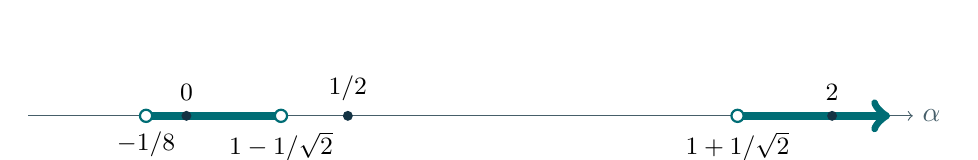
\begin{tikzpicture}[x=4.1cm,y=1cm]
\draw[->,muted] (-.49,0)--(2.25,0) node[right]{$\alpha$};
\draw[line width=3pt,teal] (-.125,0)--(.292893,0);
\draw[line width=3pt,teal,->] (1.7071,0)--(2.18,0);
\foreach \x/\t in {-.125/{-1/8},.29289/{1-1/\sqrt{2}},1.7071/{1+1/\sqrt{2}}}{\draw[teal,thick,fill=white] (\x,0) circle (2.2pt);\node[below] at (\x,-.08){\small $\t$};}
\foreach \x/\t in {0/0,.5/{1/2},2/2}{\fill[ink] (\x,0) circle (1.8pt);\node[above] at (\x,.07){\small $\t$};}
\end{tikzpicture}\end{center}
The teal intervals are computed above from the strict inequalities; the three black dots are the checks in G04.
\lead{State-matrix variant} Specify \m{'Type','matrix'} for $A_0+(tI)A_1$ or $A_0+A_1(tI)$. The same scalar $t$ does not generally commute with the entries of $A_1$. This is a fixed-ray result for a state matrix; it is not a robust test for arbitrary matrix polytopes. In discrete-time rays regularity events are tracked alongside boundary contacts. An unresolved endpoint is \m{NaN}; $\pm\infty$ and \m{NaN} mean different things.
\topic{When the physical parameter has limits}{sec:windows}
Suppose a calibration parameter is constrained to $B\subset\HH$. This box defines the \emph{admissible family}, useful for robust checks and sampling. The stable nominal law can still be deliberately studied beyond $B$. On a fixed line there are two separate questions:
\[
 J_{\rm stab}=(\alpha_-,\alpha_+),\qquad
 J_B=\{\alpha\in\RR:\alpha u\in B\}.
\]
A physical box edge is not evidence of dynamical contact. The part of the nominal stable branch that is physically allowed is $J_B\cap J_{\rm stab}$. Open and closed endpoints must be kept distinct. $J_B$ can even be empty, a singleton, or a window not containing zero.
\lab{G11}
For $p_t=s+2+t$ and $u=-2$, the polynomial on the line is $s+2-2\alpha$. It is strictly stable for $\alpha<1$. The material constraint $-3\le t\le-1$ independently gives $1/2\le\alpha\le3/2$. The physically admissible part of that stable branch is therefore $[1/2,1)$; $1/2$ is a material edge and $1$ a dynamical contact. The full-law nominal $t=0$ is outside this particular box.
\lead{A different minimization} \m{freqmargin} minimizes $|t|$ at a specified boundary frequency, over directions in quaternion space. At $s$-frequency $\omega$ in this example its answer is $\sqrt{4+\omega^2}$. The global minimum over frequency is two, attained at $t=-2$, and \m{stabilityradius} returns a numerical bracket containing it. The unrestricted calls in G11 use the two polynomials explicitly. If called with a bounded family, requesting \m{'ExtendParameter',true} explicitly asks for the unrestricted law. It does not compute a radius restricted to $B$. For state matrices, use the documented ray interface; the all-direction scalar polynomial radius is a different algorithm.
\topic{Polytopes: sample the member before taking its norm}{sec:poly}
Let $p_w=\sum_{r=1}^{m} w_r p_r$ with real barycentric weights $w_r\ge0$, $\sum w_r=1$. At complex frequency $\zeta$, take the four complex component values of each $p_r$ as a vector $v_r\in\CC^4$. The norm value of a member is
\[
 N_{p_w}(\zeta)=\sum_{r,s}w_rw_s B_{rs},\qquad B_{rs}=v_r^{\mathsf T}v_s.
\]
The transpose has \emph{no} complex conjugation. A convex hull of these polarization values contains the actual set: $w_rw_s\ge0$ sum to one. But the products are related, so most independent convex combinations of the $B_{rs}$ need not be attainable. Even the convex hull of the generator \emph{norm values} alone can miss actual member values.
\lab{G06}
Use $p_t=s+1+t\qj$, $-2\le t\le2$. At $s=0$ the actual norm values are $1+t^2$, so the exact range is $[1,5]$. The mixed control between the ends is $1-4=-3$. The global hull $[-3,5]$ contains zero, even though every actual value is positive. Each half-segment has mixed control $1$ instead, and either local hull excludes zero.
\begin{center}
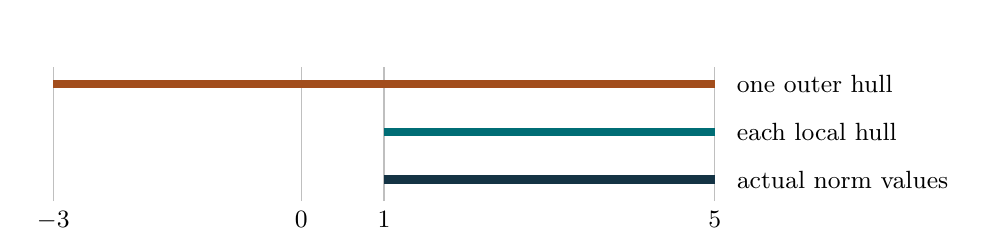
\begin{tikzpicture}[x=1.05cm,y=.55cm]
\foreach \x/\n in {-3/{-3},0/0,1/1,5/5}{\draw[black!25] (\x,0)--(\x,3.1);\node[below] at (\x,0){\small $\n$};}
\draw[line width=3pt,warm] (-3,2.7)--(5,2.7);\node[right] at (5.15,2.7){\small one outer hull};
\draw[line width=3pt,teal] (1,1.6)--(5,1.6);\node[right] at (5.15,1.6){\small each local hull};
\draw[line width=3pt,ink] (1,.5)--(5,.5);\node[right] at (5.15,.5){\small actual norm values};
\end{tikzpicture}\end{center}
In \m{valueset}, \m{Weights} uses \emph{one row per member}. In \m{valueenclosure}, each matrix in \m{VertexCells} uses \emph{one column per local vertex}, expressed in the coordinates of the original generators. A user-specified subdivision must cover the family if its union is to describe all members. This calculation proves exclusion at one frequency only.
\topic{A cubic from the polytope study}{sec:paper}
Six quaternion polynomials illustrate why a false zero in an outer hull matters for a control model. Write $A=s+1+\unit$, $B=s+3+\qk$ and let $u$ run through the four sign triples
\[
 (+,+,+),\quad(+,-,-),\quad(-,+,-),\quad(-,-,+).
\]
For the first four generators set $C_u=s+2+3(u_1\unit+u_2\qj+u_3\qk)$, $p_u=A C_u B$ \emph{in that order}. Add $p_5=p_1+AB/10$ and $p_6=p_1+s^2/10$. The polynomial product commutes with the central $s$, not with the quaternion coefficients. The short helper at the bottom of the runnable file performs polynomial convolution with ordered Hamilton products. It needs only real arithmetic; it is not a general polynomial class.
\lab{G07}
At $s=0$ each $v_r\in\RR^4$; the diagonal controls $v_r^{\mathsf T}v_r$ give the six generator values. The seventh weight row has equal weights on the first four. Their varying imaginary signs cancel \emph{before} taking the norm: the seventh value is 80, although all first four generator values are 620. In fact the seventh constant is $A(0)\,2\,B(0)$, so its squared norm is $2\cdot4\cdot10=80$.
\[
 \underbrace{620,620,620,620,628.2,620}_{\text{six generators}},\qquad
 \underbrace{80}_{\text{one admissible mixture}}.
\]
Meanwhile $B_{11}=620$ and $B_{12}=-100$. The displayed independent convex combination $5B_{11}/36+31B_{12}/36=0$ puts zero in the \emph{outer} hull. Those are weights on the controls, not weights on the original six generators. None of the seven sampled members supplies that zero. These concrete calculations explain the need for localization; they do not certify stability of this whole cubic family. The full argument is in M. Šebek, \emph{A Sharp Face Theorem for Robust Stability of Quaternionic Polynomial Polytopes} (manuscript prepared for \emph{Automatica}). The exact-data companion is separate from this finite MATLAB experiment: run \m{python reproducibility/qb03/replay.py} from the repository root to replay the mechanical and cubic rational checks. No Python installation is needed for the MATLAB guide. For package citations and publication updates see \m{docs/papers.md}.
\topic{From local evidence to a robust verdict}{sec:cert}
The zero-exclusion argument uses a connected parameter family, a strictly stable reference member, and a constant effective degree (or the corresponding forward regularity condition). Under these hypotheses a root cannot leave the open stability region without contacting its boundary. The numerical problem is to exclude the origin from the norm-value set \emph{for every boundary frequency and every admissible parameter}. Finite samples at selected frequencies cannot discharge those quantifiers.
\lead{Choose a computational route} \m{qstab.zeroexclude} subdivides a joint parameter--frequency search. For a polytope one may request \m{'Reduction','four-generator'}: the reduced tests concern whole convex hulls of up to four generators, including their interiors. This is not the classical recipe of checking only exposed edges, or a vertex stability test. It applies with the stated fixed-degree and reference requirements. The scalar \m{qstab.robuststable} also offers a Lyapunov subdivision route. Either numerical method can stop with unresolved regions.
\lab{G08}
For the first family the real root lies between $-2$ and $-1$. For the second it lies between $1$ and $2$: one admissible member is enough to refute robust stability. \m{certificateData} reads the records already retained by the solver; \m{witnessData} reconstructs a polynomial from the original family and the saved report, checks admissibility and inspects its spectrum. Do not reuse a saved witness with different generators or different coefficient bounds.
\lead{How to diagnose an undecided case}
Read \m{I.status} and \m{I.message} first. If the family can lose a required coefficient, inspect \m{qstab.leadingbound}; a zero lower estimate alone does not establish a degree-loss witness. For a path such as $1+(1-2\theta)s$, the leading coefficient is $+1$ at one end and $-1$ at the other but zero at $\theta=1/2$. Testing it only at the ends misses the problem. A degree loss is an assumption event, not a fabricated finite unstable root. If subdivision used its budget, retain the unresolved cells and increase \m{MaxTime}, \m{MaxCells} or \m{MaxDepth} only if the existing result warrants it. A larger budget can refine the answer; it does not change an assumption.
\lead{Inspect a cell} Plot the retained cells and gaps with \m{plotCertificate}. To see the geometry, \m{certificateEnclosure} reconstructs a specific stored value-space cell; \m{plotEnclosure} displays the individual outer regions. A Lyapunov slack is not a norm-value gap. A plot of accepted frequency intervals cannot by itself establish coverage of the parameter domain.
\topic{Coefficient balls and component boxes}{sec:ball}
A \emph{coefficient ball} allows a quaternion perturbation $\delta_k$ to every active coefficient. Given nonnegative real weights $\gamma_k$, its scaled size is
\[
    \left\|\big(|\delta_k|/\gamma_k\big)_{k:\gamma_k>0}\right\|_\eta ,
    \qquad 1\le\eta\le\infty .
\]
A zero weight fixes that coefficient. The quaternion directions within each coefficient are isotropic. In a \emph{component box}, the perturbations are bounded separately as $|\delta_{\nu k}|\le r W_{\nu k}$, where $W$ is a real nonnegative $4\times(g+1)$ array in the chosen coefficient basis. Now a zero width fixes just the selected component. Rotating the imaginary directions of the query can change what is attainable.
\lab{G09}
For $p=s+2$, allowing an arbitrary quaternion constant perturbation requires $|\delta_0|=|2+u|=\sqrt5$ to obtain a zero somewhere on the unit imaginary sphere. The ball query at the complex representative $\ii$ covers that \emph{whole class}. The box here varies only the real constant; forcing a zero at the specific point zero requires $\delta_{00}=-2$, hence a scale of two. These figures illustrate two explicitly different questions; they need not agree.
\lead{Why the algorithms differ} If $z=x+\ii y$ and $u^2=-1$, the right evaluation $p_r(x+u y)$ can be written $e+o u$, where $e=\sum p_k\operatorname{Re}(z^k)$ and $o=\sum p_k\operatorname{Im}(z^k)$ are quaternions. For an isotropic weighted ball the distance to the class is determined by the least singular value of $\sum_k \chi(p_k)z^k$, a $2\times2$ complex matrix, divided by the appropriate dual norm of $(\gamma_k|z|^k)_k$ when sensitive. No fixed imaginary direction needs to be guessed. For component boxes, \m{boxvalue} solves a real feasibility/gauge problem for an \emph{actual quaternion point}. Sampling a few points on a sphere does not prove a minimum over the class.
\par\smallskip\noindent\begin{tabularx}{\linewidth}{@{}p{.22\linewidth}YY@{}}\toprule
Question & Coefficient ball & Component box\\\midrule
One location & \m{ballvalue}, \m{ballset} (class membership) & \m{boxvalue} (point distance)\\
First global loss as scale increases & \m{ballradius} returns a bracket & \m{boxradius} returns a bracket\\
Specified closed scale robust? & \m{ballstable} & \m{boxstable}\\\bottomrule
\end{tabularx}\par\smallskip
A full-radius result must account for all boundary frequencies and possible loss of effective degree. If all admissible perturbations fix a component, do not replace its zero weight by a tiny positive number. Record the exponent, widths, grade, variable and termination status with a reported margin.
\topic{What does a plot in two dimensions show?}{sec:plot}
There are two different objects to display. A \emph{zero plot} computes the algebraic zero classes of each sampled member. In the plane it places each class at $(\operatorname{Re}\lambda,|\operatorname{Im}\lambda|)$. Both coordinates and the norm of the representative are exact invariants of similarity. A three-dimensional drawing of one such class at constant real part uses an exact slice of its imaginary sphere, giving a circle. Its stability does not depend on which direction on that sphere is chosen.
\par A \emph{value plot} fixes a frequency, constructs members, and then evaluates each one. Select the projection according to the question:
\par\smallskip\noindent\begin{tabularx}{\linewidth}{@{}p{.17\linewidth}Y@{}}\toprule
Projection & Coordinates; what a point at the origin means\\\midrule
\m{class} & $(\operatorname{Re}w,\|\operatorname{Im}w\|)$ for the actual evaluated quaternion $w$. It preserves $|w|$; the plotted origin means $w=0$ at the sampled point. Imaginary directions are lost.\\
\m{slice} & $(\operatorname{Re}w,\langle\operatorname{Im}w,u\rangle)$ for a fixed pure unit $u$. The omitted length is in \m{offSlice}. A dot at the origin may mean a nonzero value perpendicular to the slice.\\
\m{normpoly} & $(\operatorname{Re}N_p(\zeta),\operatorname{Im}N_p(\zeta))$ at a central complex argument. Zero is an algebraic class contact. This is not the complex projection of the physical quaternion value.\\\bottomrule
\end{tabularx}\par\smallskip
\lab{G10}
For the seeded cubic the monic leading coefficient is fixed. Each of the other three powers has four free real parts: the result has nine rows and twelve parameter columns, with no convex weights. For a two-generator polytope one would instead find two common barycentric weights per row. Inspect \m{V.sample.parameterIndex} and \m{V.coefficients(:,:,n)} to identify an actual sampled member. For a drawing of the same data, request a plot explicitly:
\begin{lstlisting}
R = qstab_guide_example('G10');
[ax,Z] = qstab.plotFamilyZeros(R.family,81);
[ax,V] = qstab.plotFamilyValues(R.family,1,81,'Projection','slice');
\end{lstlisting}
Use \m{'Sampling','grid'} for a deterministic design or \m{'Sampling','random','Seed',17} for repeatable draws. The count is the total number of sampled \emph{members}, not the number per coordinate. With a physical input axis $u$, the substitution is $u\omega$ in continuous time, $\cos\theta+u\sin\theta$ for $z$ and $\cos\theta-u\sin\theta$ for delay. Use radians per sample in discrete time. Sampled curves can be persuasive even when an unsampled member lies on the boundary.
\topic{Function directory}{sec:directory}
Use qualified names in MATLAB. Type \m{help qstab.raymargin} for its full syntax. A name by itself need not select the intended function. The tables show the mathematical return value first. Detailed argument checking, name/value options, tolerances and method-specific limits are in MATLAB help and the per-function reference pages.
\par\smallskip\noindent\begin{tabularx}{\linewidth}{@{}p{.30\linewidth}Y@{}}\toprule
Name after \m{qstab.} & Use and result\\\midrule
\m{about} & Release, numerical scope and dependencies.\\
\m{components} & Extract same-shaped real arrays $a,b,c,d$ from quaternion, complex or real data.\\
\m{polycomponents} & Extract a real $4\times(g+1)$ coefficient table; optional metadata distinguishes stored grade and actual degree.\\
\m{family} & Construct a reusable ordinary structure from an interval, polytope, affine law or shared quaternion law.\\
\m{randfamily} & Construct a random but well-defined family with a controlled degree, type and optional seed.\\
\m{familycomponents} & Inspect generator coefficients, weights or real parameter coordinates of a bounded scalar family.\\
\m{normpoly} & Real ascending coefficients of the central norm of one scalar polynomial.\\
\m{chi} & Complex adjoint of a quaternion matrix, applied coefficient by coefficient when appropriate.\\
\m{companion} & One output: normalized complex companion when possible. Two outputs: matrices of the generalized companion pencil, retaining the grade.\\
\m{roots} & Canonical complex representatives of algebraic zero classes, retaining multiplicity and infinite modes at a declared grade.\\
\m{eig}, \m{eigpairs} & Right class representatives; or $(V,D)$ and numerical residual and basis information. Not a solver for left eigenvalues.\\
\m{isstable} & Strict nominal decision for scalar polynomials or square state matrices. Its nominal square polynomial-matrix branch is experimental and has additional regularity requirements.\\
\m{lyapoperator} & Real representation of $X\mapsto AX+XA^*$ on quaternion Hermitian matrices.\\
\m{robuststable} & Whole scalar-family decision using subdivision and Lyapunov or zero-exclusion criteria.\\
\m{zeroexclude} & Whole-family numerical zero exclusion with explicit variable, budget, optional reductions and retained coverage.\\
\m{leadingbound} & Lower estimate for the norm of the required coefficient over the entire family; read the separation or witness status.\\
\m{kharitonovcube} & Continuous-time interval reduction to an affine model with eight real continuous parameters.\\\bottomrule
\end{tabularx}\par\smallskip
\clearpage
{\Large\bfseries Margins, evidence and displays}\par\medskip
\par\smallskip\noindent\begin{tabularx}{\linewidth}{@{}p{.30\linewidth}Y@{}}\toprule
Name after \m{qstab.} & Use and result\\\midrule
\m{raymargin} & First signed endpoints along a fixed quaternion direction. A prescribed parameter window is reported separately.\\
\m{freqmargin} & Smallest quaternion parameter norm for a class contact at a prescribed frequency.\\
\m{stabilityradius} & Global all-direction bracket for one shared quaternion perturbing a scalar polynomial.\\
\m{ballvalue}, \m{ballset} & Pointwise class distance and membership in a spectral set for weighted coefficient balls. Membership is not a global stability decision.\\
\m{ballradius}, \m{ballstable} & First global loss bracket and strict decision at a chosen ball size.\\
\m{boxvalue}, \m{boxradius}, \m{boxstable} & Actual-point component-box gauge, global scale bracket, and strict decision for a given scale.\\
\m{valueset} & Sample complex \emph{norm values} for chosen members and arguments. The result retains the shared weights or coordinates.\\
\m{valueenclosure} & Enclose norm values at one complex argument over a polytope or supported box/affine cell; keep the union of local regions.\\
\m{certificateData}, \m{certificateEnclosure} & Read stored coverage data; reconstruct one retained value-space enclosure, where supported.\\
\m{witnessData} & Reconstruct a particular polynomial and inspect admissibility and separate nominal diagnostics.\\
\m{plotSpectrum} & Display a supplied set of right eigenvalue or algebraic zero classes in 2D or an exact 3D slice.\\
\m{plotValueSet}, \m{plotEnclosure} & Display norm samples and separate outer regions. Show mixed controls without calling them actual family members.\\
\m{plotCertificate}, \m{plotWitness} & Display saved evidence: coverage records or a reconstructed member's classes.\\
\m{plotFamilyZeros}, \m{plotFamilyValues} & Sample actual members. Compute a cloud of algebraic zero representatives or display a class, slice or norm projection at one frequency.\\\bottomrule
\end{tabularx}\par\smallskip
\lead{Where the present release stops} Family certification concerns scalar quaternion polynomials with the documented uncertainty models. Nominal matrix and selected fixed-ray matrix routines do not constitute a robust-polynomial-matrix solver. The code uses ordinary floating point with residual, scale and separation checks; a numerical pass is not a directed-rounding interval proof. A sampled zero cloud, an outer enclosure at one frequency, a verified unstable member and a positive global numerical certificate answer four different questions. State which one you obtained when reporting a result.
\end{document}
